\documentclass[11pt, a4paper]{scrartcl}

\usepackage[english]{babel}
\usepackage[paper=a4paper,bottom=3cm,top=3cm,left=2.5cm,right=2.5cm]{geometry}
\usepackage[T1]{fontenc}
\usepackage[utf8]{luainputenc}

\usepackage{graphicx}
\usepackage{wrapfig}

\usepackage{epstopdf}
\usepackage{amsmath}
\usepackage{amsfonts}

\usepackage[backend=biber]{biblatex}
\usepackage{csquotes}
\addbibresource{Sources.bib}

\title{An Overview Of Coaxial Rotors In Helicopter Design}
\author{Bjarne Oldenburg}
\date{\today}

\begin{document}

\maketitle

\begin{center}
    Themenausarbeitung im Rahmen der Schlüsselqualifikation eines\\ \emph{\LaTeX-Einführungskures}\\ an der Universität Stuttgart.
    \vspace{1cm}\\
\end{center}

\section{Abstract\label{Abstract}}
Most helicopter models, both contemporary and historical, use a main and rear rotor configuration, in which the torque produced by the engine is counteracted
by the rear rotor. However, there exist a few models - most notably those of the Soviet/Russian Kamov Design Bureau - that use a coaxial rotor configuration instead.While this does offer benefits in engine utilization and flight behaviour, it also adds a considerable technical challenge in rotor assembly design.

\section{Introduction\label{Introduction}}
A helicopter, named so by \emph{Ponton d' Amécourt}, who derived the name from the greek \emph{elikoeioas}, meaning winding (the word helix is derived from the very same origin), and \emph{pteron}, which means wing, is - as implied by the etymological background - defined as an aircraft using rotating airfoils as means of generating lift, thrust and any control inputs, and that is capable of controlled hover without forward movement.\cite{leishman-2000} Modern day helicopters most commonly use a single rotor to generate lift. However, there are alternative options for the rotor configuration, one of which is the usage of two rotors, mounted on a single axis of rotation, driven by a common powerplant.

\section{Main\label{Main}}
The historical development of helicopters settled, after a large variety of designs in the early 1900s, on most helicopters using a larger main rotor, which generates vertical thrust and control inputs, combined with a smaller rear rotor to counteract the torque exerted on the helicopter. This has several downsides, including the reduction of engine power used to actually generate lift, since the rear rotor requires a not insubstantial amount of output - the baseline demand of a typical rotor can be as high 15\% of generated power in a hover flight.\cite{dries-2003} The logical solution to the torque generated by a single rotor is to use multiple contra-rotating rotors that cancel out each other. In early designs of the 1930s as many as 6 or 4 rotors were used,\cite{Pescara-1930} but this quickly proved impractical. Therefore, the dual-rotor coaxial design established itself as the main 

\begin{figure}
    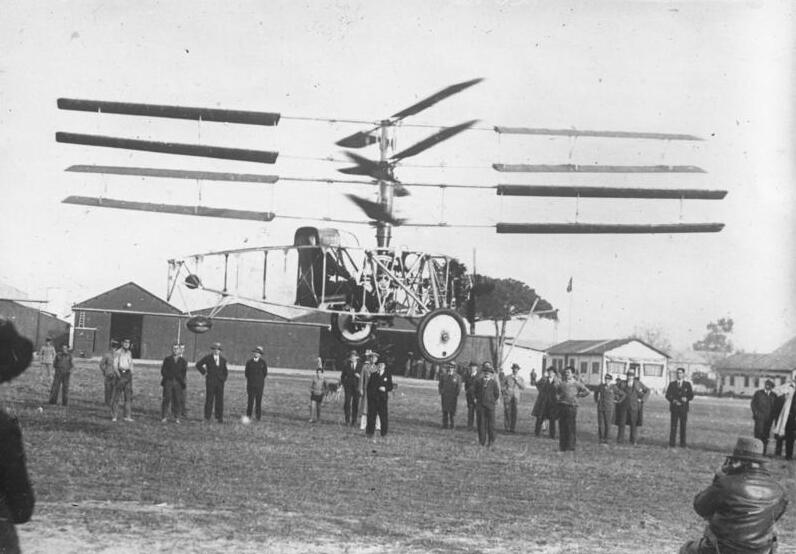
\includegraphics[width=0.5\textwidth]{Early_Coaxial.jpg}
    \caption{An early coaxial helicopter, model Pescara 4S, takes flight in Barcelona}
\end{figure}
\vspace{1cm}

\printbibliography

\end{document}